\documentclass[aps, pra, 10pt, twocolumn, superscriptaddress,floatfix]{revtex4-1}

\usepackage{amsmath,amssymb,amsfonts}
\usepackage{braket}
\usepackage[breaklinks=true,colorlinks,citecolor=blue,linkcolor=blue,urlcolor=blue]{hyperref}
\usepackage{mathtools}
\usepackage{dsfont}

%%
\def \id {\mathds{1}}
\def \abs {\text{Abs}}

\DeclareMathOperator{\tr}{Tr}

\begin{document}
%
\title{Notes on the extension of the work with Sciarrino} 
%

\author{Federico Belliardo}
\email{federico.belliardo@sns.it}
\affiliation{NEST, Scuola Normale Superiore, I-56126 Pisas,~Italy}


\maketitle

\section{Introduction}
%
A possible extension of the work done with Sciarrino is to perform an experiment with \textit{a priori} unknown visibilities and with arbitrary choice of the base of the polarization measurements on the photons. In this notes I present some approaches to this task and why I find them problematic.

\section{Extension of our algorithm}
%
The photon distribution that is used in the experiment done in collaboration with Sciarrino depends on the visibilities of all the four q-plates, that is, in order to find the number of photons $\nu_i$ to be used at the $i$-th stage we need to know in advance the visibilities of all the stages (non only the visibility of the $i$-th stage). We could perform an initial visibility estimation step followed by the phase estimation, but and alternative strategy would be to try to estimate the visibilities ``on the fly'' and adapt accordingly the strategy. The photon distribution was obtained by minimization of the Lagrangian
%
\begin{multline}
	\mathcal{L} := \frac{\pi^2}{4 b \nu_K s_K^2} + \frac{3 \pi^2}{4 s_K^2} e^{-b \nu_K} + \\  + \sum_{j=1}^{K-1} \left( \frac{2 \pi D_j}{n_{j-1} s_{j-1}}\right)^2 e^{-b\nu_j \sin^2 \left( \frac{\pi}{n_j} \right)} - \lambda \left( 2 \sum_{j=1}^{K} s_j \nu_j - N \right)\; ,
	\label{eq:lagrangianExplicited}
\end{multline}
%
the optimal photon distribution $\lbrace \nu_i \rbrace_{i=1}^K$ satisfies
%
\begin{multline}
	P_j(\nu_j, V^2_j) := \\ \frac{D_j^2}{n_{j-1}^2 s_{j-1}^2 s_j} e^{-b V_j^2 \nu_j \sin^2 \left( \frac{\pi}{n_j} \right)} V_j^2 \sin^2 \left( \frac{\pi}{n_j} \right) = \text{const.}
\end{multline}
%
The idea would be to start from $\nu_j = 0, \, \forall j$ and perform a couple of measurements (Type-$0$ and Type-$+$) for the stage $j$ having the highest $P(\nu_j, \hat{V}^2_j)$, where $\hat{V}^2_j$ is an estimator for the visibility, until we run out of resources. In this way we progressively reduce all the $P_j(\nu_j, V^2_j)$ and let them converge to close values, while simultaneously updating our knowledge of the visibilities according to the performed measurements. For the squared visibility we choose the following unbiased estimator
%
\begin{equation}
	\hat{V}^2_j := \frac{\nu_j \left[ (2 \hat{f}_0 - 1)^2 + (2 \hat{f}_+-1)^2\right] - 1}{\nu_j -1} \; ,
\end{equation}
%
where $\hat{f}_0$ and $\hat{f}_+$ are the estimator for the observed frequencies of the outcome $0$ in a Type-$0$ measurement and of the outcome of $+$ in a Type-$+$ measurement. The estimator $\hat{V}^2_j$ is not bounded in $\left[0, 1 \right]$, therefore we will actually use $\min{( \max{( \hat{V}^2_j, 0 )}, 1 )}$. The problem with this approach is that the estimator $\hat{V}^2_j$ converges very slowly to the real squared visibility. Even for $\nu_j \sim \mathcal{O} (100)$ the fluctuations in the measured visibility are wild and the selected strategy is therefore very unstable. A statistical analysis, in which the experiment is repeated many times, shows that the error doesn't converge and therefore no useful phase estimation procedure has been produced. \textbf{It has however to be noted that the distribution of resources in the iterative (and frequentist) approach to phase estimation is weakly dependent on the visibilities. That is, a small variation thereof only lightly affects the distribution. A very rough knowledge of the visibilities should be enough}. A further problem of this approach is that we would have no way of deciding at which point the strategy should be updated, that is of deciding when a new q-plates should be used. \textbf{The iterative algorithm is quite rigid and the use of the information in an adaptive fashion doesn't seem to be so easy}. This may be a reason to attack the problem with a Bayesian method, but of course this will be only an application of the Bayesian analysis already carried out by Granade~\cite{Granade2012}.
%

\section{Application of Granades Bayesian method}
%
In this second section we report the application of the Bayesian phase estimation of Granade, presented in~\cite{Granade2012}, based on a particle filter approach. With such method we can fix the number of experiment to be done, that is the number of photons used ($n = \sum_{j=1}^{K} \nu_j$), but it is harder to fix the actual number of consumed resources. For each estimation with a fixed number of used photons the number of total resources $N = \sum_{j=1}^K s_j \nu_j$ is a stochastic variable. In the following, for each number of total photons used $n$ (going from $n=10$ to $n=500$, with steps of $10$) we perform $50$ experiments and compute the RMSE of the estimation.  The associated number of total resources is the mean number of total resources used in each of the $50$ repetitions with constant $n$. We then plot the RMSE as a function of the mean number of total resources used in Fig.~\ref{fig:overHSTruevisibility2phases}. In this experiment a fixed number of particles ($n_{part} = 1000$) for the particle filter has been used, this choice might not be optimal, but a greater number of particles would make the simulation very impractical. The resampling strategy is the circular resampling. The estimation has been done by keeping the visibilities as unknown, that is, we are doing an estimation in a five dimensional space $\left(\theta, V_1, V_2, V_3, V_4 \right)$. The variance of the posterior distribution (which the Bayesian algorithm tries to optimize) has been computed accounting only for the error on the phase $\theta$, that is, the weigh matrix was $G_{ij} = 0$ for $i \neq 1, \, j \neq 1$ and $G_{11} = 1$. This makes the visibilities \textbf{nuisance parameters}. This simulation was performed with the true visibilities we have in the experiment in Rome. The RMSE of a phase estimation procedure is characterized by the presence of heavy tails in the distribution $p(\hat{\theta})$ of the estimator. There is \textbf{no guarantee} that a particle filter will approximate this tails well enough to give a reliable value for the RMSE. In the case it doesn't the RMSE is underestimated.
%
\begin{figure}[!t]
	\begin{center}
		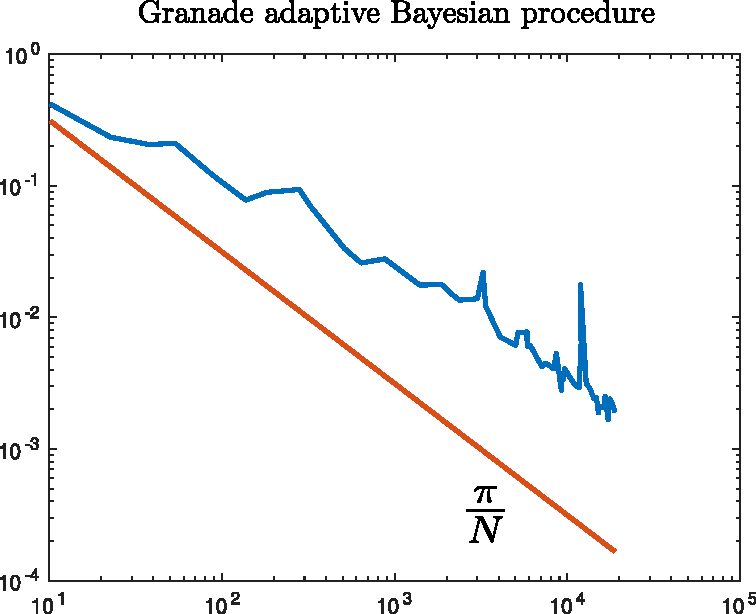
\includegraphics[width=0.45\textwidth]{overHSTruevisibility2phases.pdf}
	\end{center}
	\caption{RMSE of the Granade Bayesian estimation algorithm for $50$ repetitions of each estimation. This plot refers to a single value $\theta = 1$. The visibilities are the experimental ones. The HS line has been translated on the simulated precision.}
	\label{fig:overHSTruevisibility2phases}
\end{figure}
%
The optimal photon distribution of the Granades method seem to be actually even more unstable that the one produces with the iterative method. The reason why the error in the iterative method doesn't converge is that the this last method is not able to use efficiently the information coming from the ``wild'' photon distributions that are produced. For example if one of the advanced stages of estimation is to be done with only $\nu = 2$ measurements, this will completely spoil the iterative estimation, but not the Bayesian one. Consider two following instances of the Bayesian process with visibilities $V_j = 0.9 \; \forall j$:, where the number of measurements performed for each q-plate, and the estimated phase and visibilities are reported
%
\begin{verbatim}
	1: 76
	2: 2
	11: 59
	51: 363
	Total number of used resources: 19242
	---------------------------
	cos: 400
	sin: 100
	---------------------------
	"Phase: 2.0016"
	"V1: 0.91255"
	"V2: 0.46254"
	"V3: 0.69389"
	"V4: 0.58473"
	
	True Value: 2
\end{verbatim}
%
\begin{verbatim}
	1: 24
	2: 43
	11: 52
	51: 381
	Total number of used resources: 20113
	---------------------------
	cos: 423
	sin: 77
	---------------------------
	"Phase: 1.9999"
	"V1: 0.81227"
	"V2: 0.65486"
	"V3: 0.65035"
	"V4: 0.71512"
	
	True Value: 2
\end{verbatim}
%
The estimator for the visibilities aren't precise at all even using this Bayesian method, but this doesn't seems to be a problem for the estimation of the phase. %The number of particles used for the particles filter was $1000$, this is not particularly high, but we cannot increase too much this number otherwise the simulation becomes too long.
%There has been later work of Granade that I haven't tried to implement, the paper~\cite{Granade2012} is from 2012. It seems to me that its later should reduce the memory requirement
We also performed a Bayesian procedure where the base of the polarization measurements of the photons could be chosen in the set $\lbrace 0, \frac{\pi}{32}, \frac{2 \pi}{32}, \frac{3 \pi}{32}, \frac{4 \pi}{32}, \cdots,  \frac{\pi}{2} \rbrace$, instead of $\lbrace 0, \frac{\pi}{2} \rbrace$. The results are reported in Fig.~\ref{fig:overHS09visibility16phases}. The visibilities of this simulation were not the experimental one, instead we chose $V_j = 0.9 \; \forall j$.
%
\begin{figure}[!t]
	\begin{center}
		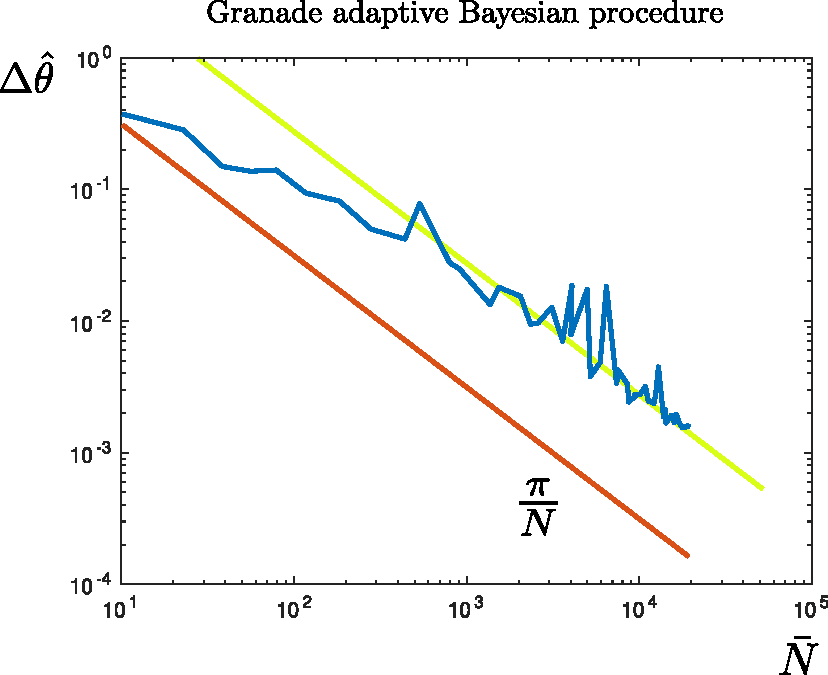
\includegraphics[width=0.45\textwidth]{overHS09visibility16phases.pdf}
	\end{center}
	\caption{RMSE of the Granade Bayesian estimation algorithm for $50$ repetitions of each estimation. This plot refers to a single value $\theta = 1$. The bases of the polarization measurements where chosen in a set of $16$ element, instead of only $2$.}
	\label{fig:overHS09visibility16phases}
\end{figure}
%

\section{Colloquium with Vittorio}
%
We should present this algorithm from Granade as an alternative to our procedure to reach the Heisenberg scaling. This method allows us to extend the estimation to a situation in which the visibilities are unknown. Not only they are unknown, but indeed they fluctuate. It is interesting to compare the results of Granade to ours by using the correct resource count.

\section{Conclusions}
%
We haven't been able to produce a functioning phase estimation procedure by modifying the iterative estimation algorithm. We could however apply the procedure given by Granade, it would be however just an application. Notice that the Bayesian procedure fails as well to determine with precision the visibilities. It turns out (as expected) that a precise knowledge of them is not very important, that is, it doesn't affect the error on the phase that much. An approximate knowledge of them is more than enough. In light of these results I don't know how significant it would be to pursue the route of performing a phase estimation experiment of this kind with nuisance visibilities since it has revealed hard to adapt our algorithm to learn the phases and the gain we can expect is anyway comparatively small.  

\begin{thebibliography}{100}
	
	\bibitem{Granade2012} C E Granade et al 2012 \href{https://doi.org/10.1088/1367-2630/14/10/103013}{New J. Phys. {\bf 14} 103013}.
	%
	
	\bibitem{Wiebe2020} T. Ramakrishna and N. Wiebe, \href{http://arxiv.org/abs/2009.07898}{http://arxiv.org/abs/2009.07898}.
	%
	
\end{thebibliography}

\end{document}